\section{ Hypyn suunnittelu }
\label{hypyn-lapikayminen-maassa-hypyn-suunnittelu}


Hyppy kannattaa suunnitella ja valita huolella etukäteen ja harjoitteluun tulee varata riittävästi aikaa. Samalla kannattaa miettiä myös hypyn tavoitteet, eli se, mitä halutaan oppia ja/tai harjoitella. Hypyn suunnittelussa ja tavoitteiden asettelussa tulee huomioida hyppääjien kokemustaso. Tavoitteena voi olla esim. asentoharjoittelu, oppia liikkumaan tarkemmin tai pitämään katsekontakti. Kuvaajaa kannattaa käyttää jokaisella hypyllä. Kaikki FS-hyppääminen perustuu perusasioiden hallintaan ja monimutkaiselta näyttävästä FS-hypystä pystyy löytämään jo oppilasaikana opetetut perusliikkeet. Oikotietä onneen ei ole eikä vauhti korjaa virheitä. 


\begin{Figure}\centering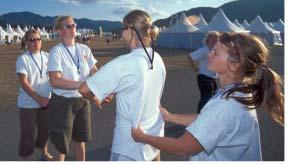
\includegraphics[width=0.95\textwidth]{Neliway-maassa.jpeg}\captionof{figure}{4-way pystykuivat}\end{Figure} 

\section{ Pystykuivat }
\label{hypyn-lapikayminen-maassa-pystykuivat}


Pystykuivien aikana pyritään oppimaan hypyn kulku eli otteet ja muodostelmat. Pystykuivilla harjoitellaan muodostelmien, oikeiden otteiden ja oman paikan muistamista. Pystykuivia toistetaan riittävän kauan, jotta kaikki muistavat hypyn kulun. Pystykuivat ovat helppo, nopea ja fyysisesti kevyt tapa harjoitella hyppyä. 

\section{ Uloshyppyharjoittelu }
\label{hypyn-lapikayminen-maassa-uloshyppyharjoittelu}


Uloshypyn toteutus riippuu hyppääjien määrästä ja hyppykoneesta, mutta onnistuakseen uloshypyn täytyy aina olla yhdenaikainen ja hyppääjien lähtöasennon ilmavirran mukainen. Yhdenaikaisuus saadaan merkinannolla, jonka voi aloittaa kun kaikki hyppääjät ovat valmiina otteet otettuina ja liikkumatta ovella. Yksi hyppääjistä aloittaa merkinannon (ready), johon muut tulevat mukaan (set - go), esim. ravistus (ready), liike sisään (set) ja ulos (go). 


Oikea lähtöasento eli vatsan kääntäminen kohti suhteellista ilmavirtaa mahdollistaa hyvän lentoasennon heti uloshypystä lähtien. Jos sekä lähtöasento että yhdenaikaisuus epäonnistuvat, ei uloshyppy onnistu. Uloshyppyä tulee harjoitella yhtä paljon kuin muodostelmia, koska onnistunut hyppy alkaa hyvästä uloshypystä. Uloshypyn merkinantoa, kiipeämistä ja asentoa ilmavirtaan harjoitellaan joko lentokoneen ovella tai konemallilla, jonka oviaukon tulisi vastata todellista ovea mahdollisimman hyvin. Uloshyppyharjoitteluun maassa kannattaa panostaa, koska uloshypyn voi suorittaa vain kerran yhdellä hypyllä. 

\section{ Lautakuivat }
\label{hypyn-lapikayminen-maassa-lautakuivat}


Lautakuivien tarkoitus on hypyn tarkempi harjoittelu maassa. Lautakuivilla hiotaan siirtymät muodostelmien välillä. Yksittäistä siirtymää harjoitellaan monta kertaa peräkkäin, tavoitteena tehdä liikkeestä mahdollisimman lyhyt ja tehokas. Toistamalla liikettä riittävästi, se pyritään saamaan lihasmuistiin. Kun muodostelmien väliset siirtymät on harjoiteltu erikseen, ne yhdistetään hyppykokonaisuudeksi. Siirtymien lisäksi lautakuivilla käydään läpi oikeat otteet, muodostelmien purkajat sekä katseiden suunnat. 


Lautakuivien rytmin ja liikkumisen tulisi olla realistista haluttuun suoritukseen nähden. Hyppyä harjoitellaan maassa kunnes kaikki tietävät ja osaavat sen. Mikä maassa on epäselvää ja vaikeaa, on se sitä myös ilmassa. Ennen koneeseen menoa kannattaa hyppy vielä kerrata pystykuivien avulla ja kiinnittää huomiota lautakuivilla läpi käytyihin asioihin. 

\section{ Jälkikuivat }
\label{hypyn-lapikayminen-maassa-jalkikuivat}


Jälkikuivissa käydään hyppysuoritus läpi suhteutettuna asetettuihin tavoitteisiin. Täyttyivätkö tavoitteet? Miltä osin? Mitä jäi puuttumaan? Mitkä asiat onnistuivat? Mitä voisi vielä parantaa? Ennen mahdollisen videon katsomista käydään läpi jokaisen muistikuvat ja havainnot hypyltä. Hypyn purkaminen mielikuvien avulla kehittää muistia ja kykyä nähdä asioita ilmassa. 


Videolta katsotaan ensin kokonaisuutta ja yksittäisiä suorituksia sen jälkeen. Videolta nähdään, ovatko lautakuivilla harjoitellut liikkeet ja tekniikat toteutuneet kuten oli suunniteltu ja vastasivatko mielikuvat hypyltä videota. Perusteellisten jälkikuivien jälkeen seuraavien hyppyjen tavoitteiden asettelu on selkeämpää. 


Jälkikuivien tarkoitus on löytää hypyllä esiintyneet ongelmat ja ne asiat, joita täytyy harjoitella tulevilla hypyillä. Toinen erittäin tärkeä tarkoitus on nostaa esiin onnistuneet suoritukset hypyltä ja palauttaa mieleen miten ne tehtiin. Täysin epäonnistunutta, huonoa hyppyä ei ole. Kaikista hypyistä löytyy onnistuneita suorituksia, olivat ne sitten kuinka pieniä tahansa. 

